\documentclass[10pt,a4paper]{report}
\usepackage[utf8]{inputenc}
\usepackage[T1]{fontenc}
\usepackage{amsmath}
\usepackage{amsfonts}
\usepackage{amssymb}
\usepackage{graphicx}
\usepackage{subfloat}
\usepackage{subfig}
%\usepackage{xcolor}
\usepackage[dvipsnames]{xcolor}
\begin{document}
	\chapter{Version}
	This document is a common guide but it applies mainly to version $12$ or $v12$.
	
	\chapter{Components}
	\begin{figure}
		\subfloat[]{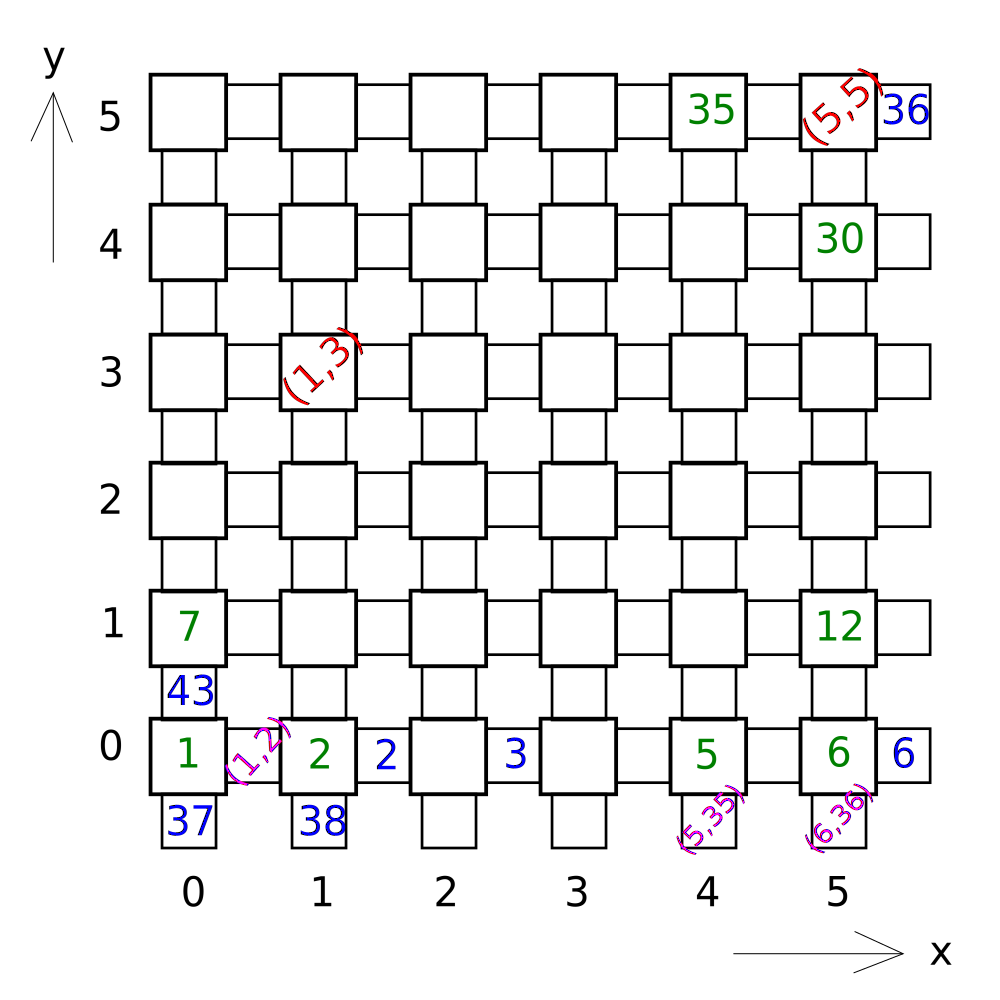
\includegraphics[width=0.8\linewidth]{fig/lattice-2.png}}
		\caption{\textcolor{red}{Red} color is for site index, \textcolor{ForestGreen}{Green} color is for site id(or label), \textcolor{magenta}{Magenta} color is for bond index, \textcolor{blue}{Blue} color is for bond id (or label).}
	\end{figure}
	\section{Site}
	\begin{enumerate}
		\item $id$ or $label$
		\item $group\_id$
		\item Index
		\item Relative Index with respect to 
	\end{enumerate}
	\section{Bond}
\begin{enumerate}
	\item $id$ or $label$
	\item $group\_id$ which can coincide with site group id
	
	\item Index. $(a,b)$ where $a$ is the $id$ of one site and $b$ is the id of another site.
\end{enumerate}
\newpage
	\section{Lattice}
	We will study $2D$ system specifically with a $2d$ vector in C++.
	\begin{enumerate}
		\item Site
		\item Bond
	\end{enumerate}
	
	A $1d$ vector looks like
	\begin{equation*}
	V_i = 
	\left[
	\begin{tabular}{c}
		0 \\ 1 \\ 2
	\end{tabular}
	\right]
	\end{equation*}
	
		A $2d$ vector looks like
	\begin{equation*}
	V_{i,j} = 
	\left[
	\begin{tabular}{cccc}
	0,0 & 0,1 & 0,2 \\
	1,0 & 1,1 & 1,2 \\
	2,0 & 2,1 & 2,2
	\end{tabular}
	\right]
	\end{equation*}
	
	But we want grid like structure 
	\begin{equation*}
	V^\prime_{i,j} = 
	\left[
	\begin{tabular}{cccc}
	0,2 & 1,2 & 2,2 \\
	0,1 & 1,1 & 2,1 \\
	0,0 & 1,0 & 2,0
	\end{tabular}
	\right]
	\end{equation*}
	where each column of $V^\prime$ is row of $V$ but backwards. So when viewing the lattice we just need to generate row index backward and  switch row and column index. Note that horizontal bonds become vertical and vice versa in this process.

	\section{Cluster}
\end{document}